% Options for packages loaded elsewhere
\PassOptionsToPackage{unicode}{hyperref}
\PassOptionsToPackage{hyphens}{url}
\PassOptionsToPackage{dvipsnames,svgnames*,x11names*}{xcolor}
%
\documentclass[
  a4paper, 12pt]{article}
\usepackage{lmodern}
\usepackage{amssymb,amsmath}
\usepackage{ifxetex,ifluatex}
\ifnum 0\ifxetex 1\fi\ifluatex 1\fi=0 % if pdftex
  \usepackage[T1]{fontenc}
  \usepackage[utf8]{inputenc}
  \usepackage{textcomp} % provide euro and other symbols
\else % if luatex or xetex
  \usepackage{unicode-math}
  \defaultfontfeatures{Scale=MatchLowercase}
  \defaultfontfeatures[\rmfamily]{Ligatures=TeX,Scale=1}
\fi
% Use upquote if available, for straight quotes in verbatim environments
\IfFileExists{upquote.sty}{\usepackage{upquote}}{}
\IfFileExists{microtype.sty}{% use microtype if available
  \usepackage[]{microtype}
  \UseMicrotypeSet[protrusion]{basicmath} % disable protrusion for tt fonts
}{}
\makeatletter
\@ifundefined{KOMAClassName}{% if non-KOMA class
  \IfFileExists{parskip.sty}{%
    \usepackage{parskip}
  }{% else
    \setlength{\parindent}{0pt}
    \setlength{\parskip}{6pt plus 2pt minus 1pt}}
}{% if KOMA class
  \KOMAoptions{parskip=half}}
\makeatother
\usepackage{xcolor}
\IfFileExists{xurl.sty}{\usepackage{xurl}}{} % add URL line breaks if available
\IfFileExists{bookmark.sty}{\usepackage{bookmark}}{\usepackage{hyperref}}
\hypersetup{
  pdftitle={Modelos hierárquicos na Engenharia de Avaliações},
  pdfauthor={Luiz F. P. Droubi; Carlos Augusto Zilli; Norberto Hoccheim},
  colorlinks=true,
  linkcolor=red,
  filecolor=Maroon,
  citecolor=green,
  urlcolor=magenta,
  pdfcreator={LaTeX via pandoc}}
\urlstyle{same} % disable monospaced font for URLs
\usepackage[left=2.5cm,right=2.0cm,top=1.5cm,bottom=1.5cm]{geometry}
\usepackage{longtable,booktabs}
% Correct order of tables after \paragraph or \subparagraph
\usepackage{etoolbox}
\makeatletter
\patchcmd\longtable{\par}{\if@noskipsec\mbox{}\fi\par}{}{}
\makeatother
% Allow footnotes in longtable head/foot
\IfFileExists{footnotehyper.sty}{\usepackage{footnotehyper}}{\usepackage{footnote}}
\makesavenoteenv{longtable}
\usepackage{graphicx,grffile}
\makeatletter
\def\maxwidth{\ifdim\Gin@nat@width>\linewidth\linewidth\else\Gin@nat@width\fi}
\def\maxheight{\ifdim\Gin@nat@height>\textheight\textheight\else\Gin@nat@height\fi}
\makeatother
% Scale images if necessary, so that they will not overflow the page
% margins by default, and it is still possible to overwrite the defaults
% using explicit options in \includegraphics[width, height, ...]{}
\setkeys{Gin}{width=\maxwidth,height=\maxheight,keepaspectratio}
% Set default figure placement to htbp
\makeatletter
\def\fps@figure{htbp}
\makeatother
\setlength{\emergencystretch}{3em} % prevent overfull lines
\providecommand{\tightlist}{%
  \setlength{\itemsep}{0pt}\setlength{\parskip}{0pt}}
\setcounter{secnumdepth}{5}
\usepackage[brazil]{babel}
\usepackage{graphicx}
\usepackage{float}
\usepackage{subfig}
\usepackage{caption}
\usepackage{lastpage}
\usepackage{rotating}
\usepackage{mathrsfs}
\usepackage{bm}
\usepackage{dcolumn}
\setlength{\parindent}{1.25cm} % Default is 15pt.
\usepackage{indentfirst}
% \usepackage{helvet}
% \renewcommand{\familydefault}{\sfdefault}
% \usepackage{newtxtext,newtxmath} % mais nova para Times.
\usepackage{mathptmx} % para Times New Roman (preferível newtxtext)
% \usepackage{Times} % para Times New Roman (obsoleto)
% \usepackage{fontspec} % para Arial e/ou Times (xelatex ou luatex)
% \setmainfont{Arial}
\newcommand{\pkg}[1]{{\normalfont\fontseries{b}\selectfont #1}}
\let\proglang=\textsf
\let\code=\texttt
\usepackage{fancyhdr}
% Turn on the style
\pagestyle{fancy}
% Clear the header and footer
\fancyhead{}
\fancyfoot{}
% Set the right side of the footer to be the page number
\fancyfoot[R]{\thepage~/~\pageref{LastPage}}
\usepackage{booktabs}
\usepackage{longtable}
\usepackage{array}
\usepackage{multirow}
\usepackage{wrapfig}
\usepackage{float}
\usepackage{colortbl}
\usepackage{pdflscape}
\usepackage{tabu}
\usepackage{threeparttable}
\usepackage{threeparttablex}
\usepackage[normalem]{ulem}
\usepackage{makecell}
\usepackage{xcolor}

\title{Modelos hierárquicos na Engenharia de Avaliações}
\usepackage{etoolbox}
\makeatletter
\providecommand{\subtitle}[1]{% add subtitle to \maketitle
  \apptocmd{\@title}{\par {\large #1 \par}}{}{}
}
\makeatother
\subtitle{Para confecção de PVG's e índices de mercado}
\author{Luiz F. P. Droubi \and Carlos Augusto Zilli \and Norberto Hoccheim}
\date{20/08/2020}

\begin{document}
\maketitle

\hypertarget{introduuxe7uxe3o}{%
\section{Introdução}\label{introduuxe7uxe3o}}

\hypertarget{revisuxe3o-bibliogruxe1fica}{%
\section{Revisão Bibliográfica}\label{revisuxe3o-bibliogruxe1fica}}

\hypertarget{estudo-de-caso}{%
\section{Estudo de Caso}\label{estudo-de-caso}}

\hypertarget{criauxe7uxe3o-de-dados-via-simulauxe7uxe3o}{%
\subsection{Criação de dados via
simulação}\label{criauxe7uxe3o-de-dados-via-simulauxe7uxe3o}}

Foram criados 550 dados de lotes, divididos igualmente em 11 bairros, a
partir de simulação com o auxílio do software \textbf{R}.

Os dados foram criados conforme parâmetros da tabela 1:

\begin{longtable}[]{@{}lrcrc@{}}
\toprule
\begin{minipage}[b]{0.18\columnwidth}\raggedright
Variável\strut
\end{minipage} & \begin{minipage}[b]{0.12\columnwidth}\raggedleft
Tipo\strut
\end{minipage} & \begin{minipage}[b]{0.11\columnwidth}\centering
Distribuição\strut
\end{minipage} & \begin{minipage}[b]{0.25\columnwidth}\raggedleft
Parâmetros\strut
\end{minipage} & \begin{minipage}[b]{0.21\columnwidth}\centering
Obs\strut
\end{minipage}\tabularnewline
\midrule
\endhead
\begin{minipage}[t]{0.18\columnwidth}\raggedright
Área (\(A\))\strut
\end{minipage} & \begin{minipage}[t]{0.12\columnwidth}\raggedleft
Quantitativa\strut
\end{minipage} & \begin{minipage}[t]{0.11\columnwidth}\centering
Normal\strut
\end{minipage} & \begin{minipage}[t]{0.25\columnwidth}\raggedleft
\(\mu = 400, \sigma = 50\)\strut
\end{minipage} & \begin{minipage}[t]{0.21\columnwidth}\centering
-\strut
\end{minipage}\tabularnewline
\begin{minipage}[t]{0.18\columnwidth}\raggedright
Bairro\strut
\end{minipage} & \begin{minipage}[t]{0.12\columnwidth}\raggedleft
Qualitativa\strut
\end{minipage} & \begin{minipage}[t]{0.11\columnwidth}\centering
-\strut
\end{minipage} & \begin{minipage}[t]{0.25\columnwidth}\raggedleft
A a K\strut
\end{minipage} & \begin{minipage}[t]{0.21\columnwidth}\centering
-\strut
\end{minipage}\tabularnewline
\begin{minipage}[t]{0.18\columnwidth}\raggedright
Áreas Verdes (\(A_V\))\strut
\end{minipage} & \begin{minipage}[t]{0.12\columnwidth}\raggedleft
Quantitativa\strut
\end{minipage} & \begin{minipage}[t]{0.11\columnwidth}\centering
Uniforme\strut
\end{minipage} & \begin{minipage}[t]{0.25\columnwidth}\raggedleft
\(\mu = 0,2 \quad a \quad 0,70\)\strut
\end{minipage} & \begin{minipage}[t]{0.21\columnwidth}\centering
Um valor para cada bairro\strut
\end{minipage}\tabularnewline
\begin{minipage}[t]{0.18\columnwidth}\raggedright
\(\beta_{0}\)\strut
\end{minipage} & \begin{minipage}[t]{0.12\columnwidth}\raggedleft
Coeficiente\strut
\end{minipage} & \begin{minipage}[t]{0.11\columnwidth}\centering
Discreta\strut
\end{minipage} & \begin{minipage}[t]{0.25\columnwidth}\raggedleft
2000\strut
\end{minipage} & \begin{minipage}[t]{0.21\columnwidth}\centering
-\strut
\end{minipage}\tabularnewline
\begin{minipage}[t]{0.18\columnwidth}\raggedright
\(\upsilon\)\strut
\end{minipage} & \begin{minipage}[t]{0.12\columnwidth}\raggedleft
Termo de erro\strut
\end{minipage} & \begin{minipage}[t]{0.11\columnwidth}\centering
Normal\strut
\end{minipage} & \begin{minipage}[t]{0.25\columnwidth}\raggedleft
\(\mu = 0, \sigma = 150\)\strut
\end{minipage} & \begin{minipage}[t]{0.21\columnwidth}\centering
-\strut
\end{minipage}\tabularnewline
\begin{minipage}[t]{0.18\columnwidth}\raggedright
\(\beta_{0j}\)\strut
\end{minipage} & \begin{minipage}[t]{0.12\columnwidth}\raggedleft
Coeficiente\strut
\end{minipage} & \begin{minipage}[t]{0.11\columnwidth}\centering
Não definida\strut
\end{minipage} & \begin{minipage}[t]{0.25\columnwidth}\raggedleft
\(\beta_0 + 3000A_V + \upsilon\)\strut
\end{minipage} & \begin{minipage}[t]{0.21\columnwidth}\centering
-\strut
\end{minipage}\tabularnewline
\begin{minipage}[t]{0.18\columnwidth}\raggedright
\(\epsilon\)\strut
\end{minipage} & \begin{minipage}[t]{0.12\columnwidth}\raggedleft
Termo de erro\strut
\end{minipage} & \begin{minipage}[t]{0.11\columnwidth}\centering
Normal\strut
\end{minipage} & \begin{minipage}[t]{0.25\columnwidth}\raggedleft
\(\mu = 0, \sigma = 50\)\strut
\end{minipage} & \begin{minipage}[t]{0.21\columnwidth}\centering
-\strut
\end{minipage}\tabularnewline
\begin{minipage}[t]{0.18\columnwidth}\raggedright
Valor Unitário (\(VU\))\strut
\end{minipage} & \begin{minipage}[t]{0.12\columnwidth}\raggedleft
Quantitativa\strut
\end{minipage} & \begin{minipage}[t]{0.11\columnwidth}\centering
Não definida\strut
\end{minipage} & \begin{minipage}[t]{0.25\columnwidth}\raggedleft
\(\beta_{0j} - 3,0 A + \epsilon\)\strut
\end{minipage} & \begin{minipage}[t]{0.21\columnwidth}\centering
-\strut
\end{minipage}\tabularnewline
\bottomrule
\end{longtable}

\hypertarget{anuxe1lise-exploratuxf3ria-dos-dados}{%
\subsection{Análise exploratória dos
dados}\label{anuxe1lise-exploratuxf3ria-dos-dados}}

Na figura \ref{fig:exploratoria} é possível ver os principais gráficos
dos dados gerados.

\begin{figure}[H]

{\centering 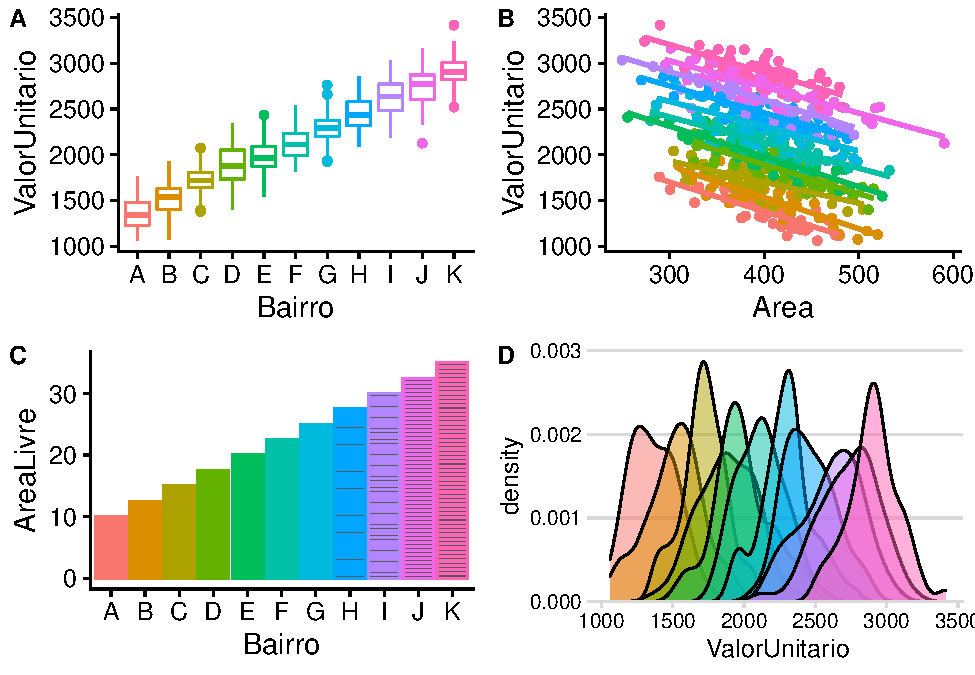
\includegraphics[width=1\linewidth]{EstudoCaso_files/figure-latex/exploratoria-1} 

}

\caption{Análise exploratória dos dados.}\label{fig:exploratoria}
\end{figure}

\hypertarget{ajuste-de-modelos}{%
\subsection{Ajuste de modelos}\label{ajuste-de-modelos}}

Com os dados gerados foram ajustados um modelo de efeitos fixos e três
modelos mistos: um modelo misto simples, que praticamente equivale ao
modelo de efeitos fixos, um modelo misto com a adição de uma variável de
segundo nível e um modelo misto utilizando-se a formulação de Mundlak.

Para o ajuste do modelo de efeitos fixos foram utilizados todos os dados
gerados, pois não há como prever valores para bairros não contemplados
na amostra em um modelo deste tipo.

Para o ajuste dos modelos mistos foram removidos os 50 dados relativos
ao bairro H, que foram reservados para serem utilizados posteriormente
para validação dos modelos, mostrando como a previsão de valores em
modelos de efeitos mistos pode ser feita para agrupamentos não
contemplados na amostra.

\hypertarget{modelo-de-efeitos-fixos}{%
\subsubsection{Modelo de efeitos fixos}\label{modelo-de-efeitos-fixos}}

Com os dados gerados, foi elaborado um modelo de efeitos fixos, do tipo:

\[ValorUnitario = \beta_0 + \beta_1Area + \beta_{2i}Bairro_i + \epsilon\]
onde \(\beta_{2i}\) são os coeficientes das variáveis dicotômicas em
grupo (\(Bairro_i\)).

\hypertarget{modelo-misto-simples}{%
\subsubsection{Modelo misto simples}\label{modelo-misto-simples}}

Também foi elaborado um modelo misto do tipo:

\[ValorUnitario = \beta_0 + \beta_1Area + \upsilon_i + \epsilon\] Onde
\(\upsilon_i\) é uma variável aleatória que foi utilizada para modelar
os diferentes bairros.

Os efeitos aleatórios do modelo misto simples podem ser visualizados na
Figura \ref{fig:dotplot}.

Como se pode notar na Figura \ref{fig:dotplot}, os valores dos
interceptos aleatórios para cada bairro giram em torno de zero, o seu
valor médio. Como o Bairro H (com \(A_L = 0,55\)) foi omitido no ajusto
do modelo, não há valores estimados para os efeitos aleatórios para este
bairro.

\begin{figure}[H]

{\centering 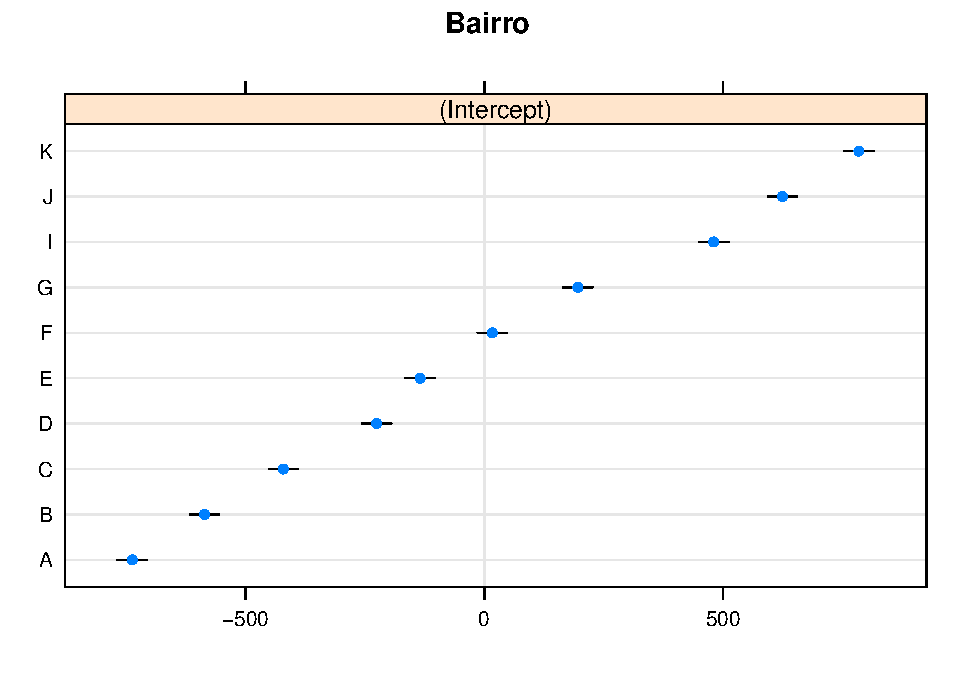
\includegraphics[width=0.7\linewidth]{EstudoCaso_files/figure-latex/dotplot-1} 

}

\caption{Efeitos aleatórios do modelo.}\label{fig:dotplot}
\end{figure}

Os valores de referência para cada bairro podem ser obtidos através da
soma do intercepto global do modelo misto simples com os interceptos
aleatórios, o que pode ser visto na tabela \ref{tab:somaitcpt}.

\begin{table}

\caption{\label{tab:somaitcpt}Valores dos interceptos para cada bairro.}
\centering
\fontsize{10}{12}\selectfont
\begin{tabular}[t]{lrrrrrrrrrr}
\toprule
  & A & B & C & D & E & F & G & I & J & K\\
\midrule
(Intercept) & 2.579,7 & 2.730,8 & 2.895,8 & 3.091 & 3.181,9 & 3.333 & 3.512,2 & 3.796,2 & 3.940 & 4.100\\
\bottomrule
\end{tabular}
\end{table}

Como se pode perceber, quase não houve diferença entre os valores
estimados em cada modelo.

A ínica informação a mais que se pode extrair do modelo de efeitos
mistos é a componente de variância devido à localidade, separada da
variância ao nível dos imóveis, o que pode ser visto na tabela
\ref{tab:variancias}.

\begin{table}

\caption{\label{tab:variancias}Efeitos randômicos do modelo misto.}
\centering
\begin{tabular}[t]{lrr}
\toprule
grp & vcov & sdcor\\
\midrule
\rowcolor{gray!6}  Bairro & 240.555,13 & 490,46\\
Residual & 12.105,17 & 110,02\\
\bottomrule
\end{tabular}
\end{table}

Pode-se notar que a variância devido à localidade é relevante para o
modelo, haja vista que a variância devido à localidade é maior do que a
variância devido às características dos imóveis.

\hypertarget{modelo-misto-com-variuxe1veis-de-segundo-nuxedvel}{%
\subsubsection{Modelo misto com variáveis de segundo
nível}\label{modelo-misto-com-variuxe1veis-de-segundo-nuxedvel}}

Finalmente, foi elaborado um modelo misto do tipo:

\[ValorUnitario = \beta_0 + \beta_1Area + \beta_2 A_V+ \upsilon_i + \epsilon\]

Onde \(A_V\) é uma variável de nível 2 que representa a porcentagem de
áreas verdes em cada bairro, em relação à área total.

\hypertarget{modelo-misto-com-formulauxe7uxe3o-de-mundlak}{%
\subsubsection{Modelo misto com formulação de
Mundlak}\label{modelo-misto-com-formulauxe7uxe3o-de-mundlak}}

Finalmente, foi ajusta um modelo com a formulação de Mundlak. Este
modelo foi elaborado de acordo com a seguinte formulação:

\[ValorUnitario = \beta_0 + \beta_1 Area + \beta_{1C} \overline{Area}+ \beta_2 A_V+ \upsilon_i + \epsilon\]

\hypertarget{resultados}{%
\subsection{Resultados}\label{resultados}}

A tabela \ref{tab:fits} mostra as estatísticas básicas dos diversos
modelos mistos (colunas (2), (3) e (4)) comparados aos modelo de efeitos
fixos (coluna (1)).

Como pode ser vistos nesta tabela, o valor do intercepto global (a dita
grande média) foi melhor estimada (comparando-se com o valor simulado)
pelo modelo misto com a variável de segundo nível \(A_L\), obtendo um
resultado de R\$ 1.987,28. Isto ocorre porque o efeito da variável
relevante \(A_V\) não inclusa no modelo anterior havia sido absorvida
por este coeficiente.

Nos modelos onde houve a inclusão da variável Área Livre (\(A_L\)), seu
coeficiente foi bem estimado: o valor da influência das áreas verdes,
simulado como aumento R\$ 30,00/m2 a cada ponto percentual a mais de
áreas verdes no bairro do imóvel, foi precisamente estimado.

Para o modelo de Mundlak, a estimação do coeficiente contextual
(\(\beta_{1C}\)) foi insignificante. Isto era esperado, dado que a
variável Área foi simulada da mesma maneira para todos os bairros. Em
outras palavras, a simulação foi feita como se os imóveis em todos os
bairros tivessem a mesma distribuição (normal) com mesma média e
desvio-padrão. Isto dificilmente ocorrerá na prática da elaboração de
PVG's, mas é interessante notar a flexibilidade deste tipo de
formulação: quando não existe na realidade o efeito esperado pela
formulação, o coeficiente resultará insignificante. Diz-se em
estatística que o modelo degenerou, ou seja, o modelo com a formulação
de Mundlak se degenerou para uma formulação mais simples. Basta remover
este termo da modelagem para obter-se o modelo mais correto para o caso.
Portanto, na prática, deve-se partir da formulação mais complexa, no
caso a de Mundlak, e observar se os resultados obtidos são
significantes. Caso positivo, mantem-se o modelo. Caso contrário,
descarta-se o termo insignificante.

Por último, porém não menos relevante, percebe-se que este modelo tem
critérios de informação de Akaike (AIC) e de Bayes (BIC) melhores que os
dois modelos iniciais.

\begin{table}[H] \centering 
  \caption{Comparacão dos modelos de  efeitos fixos e efeitos mistos.} 
  \label{tab:fits} 
\scriptsize 
\begin{tabular}{@{\extracolsep{5pt}}lcccc} 
\\[-1.8ex]\hline 
\hline \\[-1.8ex] 
 & \multicolumn{4}{c}{\textit{Dependent variable:}} \\ 
\cline{2-5} 
\\[-1.8ex] & \multicolumn{4}{c}{ValorUnitario} \\ 
\\[-1.8ex] & \textit{OLS} & \multicolumn{3}{c}{\textit{linear}} \\ 
 & \textit{} & \multicolumn{3}{c}{\textit{mixed-effects}} \\ 
\\[-1.8ex] & (1) & (2) & (3) & (4)\\ 
\hline \\[-1.8ex] 
 Constant &  & 3.316,04 (160,12)$^{***}$ & 1.987,28 (43,75)$^{***}$ & 1.858,21 (597,46)$^{***}$ \\ 
  Area & $-$2,99 (0,09)$^{***}$ & $-$3,00 (0,10)$^{***}$ & $-$3,00 (0,10)$^{***}$ & $-$3,00 (0,10)$^{***}$ \\ 
  BairroA & 2.577,39 (40,67)$^{***}$ &  &  &  \\ 
  BairroB & 2.728,65 (40,75)$^{***}$ &  &  &  \\ 
  BairroC & 2.893,84 (39,59)$^{***}$ &  &  &  \\ 
  BairroD & 3.089,23 (40,57)$^{***}$ &  &  &  \\ 
  BairroE & 3.180,19 (40,11)$^{***}$ &  &  &  \\ 
  BairroF & 3.331,46 (40,63)$^{***}$ &  &  &  \\ 
  BairroG & 3.510,80 (40,71)$^{***}$ &  &  &  \\ 
  BairroH & 3.655,00 (40,22)$^{***}$ &  &  &  \\ 
  BairroI & 3.795,18 (39,72)$^{***}$ &  &  &  \\ 
  BairroJ & 3.939,05 (40,43)$^{***}$ &  &  &  \\ 
  BairroK & 4.099,23 (39,98)$^{***}$ &  &  &  \\ 
  Area\_between &  &  &  & 0,32 (1,48) \\ 
  AreaLivre &  &  & 3.018,16 (38,65)$^{***}$ & 3.021,14 (43,42)$^{***}$ \\ 
 \hline \\[-1.8ex] 
Observations & 550 & 500 & 500 & 500 \\ 
R$^{2}$ & 1,00 &  &  &  \\ 
Log Likelihood &  & $-$3.094,33 & $-$3.055,32 & $-$3.054,02 \\ 
Akaike Inf. Crit. & 6.734,21 & 6.196,66 & 6.120,65 & 6.120,04 \\ 
Bayesian Inf. Crit. & 6.790,23 & 6.213,51 & 6.141,72 & 6.145,33 \\ 
Residual Std. Error & 108,90 (df = 538) &  &  &  \\ 
F Statistic & 18.776,45$^{***}$ (df = 12; 538) &  &  &  \\ 
\hline 
\hline \\[-1.8ex] 
\textit{Note:}  & \multicolumn{4}{r}{$^{*}$p$<$0,3; $^{**}$p$<$0,2; $^{***}$p$<$0,1} \\ 
\end{tabular} 
\end{table}

\hypertarget{previsuxe3o-de-valores}{%
\subsection{Previsão de Valores}\label{previsuxe3o-de-valores}}

Na Figura \ref{fig:powerPlots} podem ser vistos os gráficos de poder de
predição para o modelo de efeitos fixos (A), para o modelo misto simples
(B), para o modelo misto com a variável de segundo nível (C) e para o
modelo misto com formulação de Mundlak (D). Como pode ser visto, todos
os modelos possuem poderes de predição praticamente equivalentes, com
exceção do modelo misto simples, onde a previsão de valores não pode ser
feita com precisão já que, como no modelo de efeitos fixos, este modelo
não tem parâmetros para prever valores em bairros não contemplados na
amostra. Para efetuar as previsões no bairro H, então, o modelo
considerou para a variável aleatória \(\upsilon\) o valor zero, ou seja,
o valor esperado da variável, o que levou a previsões incorretas em
relação aos valores simulados para aquele bairro.

\begin{figure}[H]

{\centering 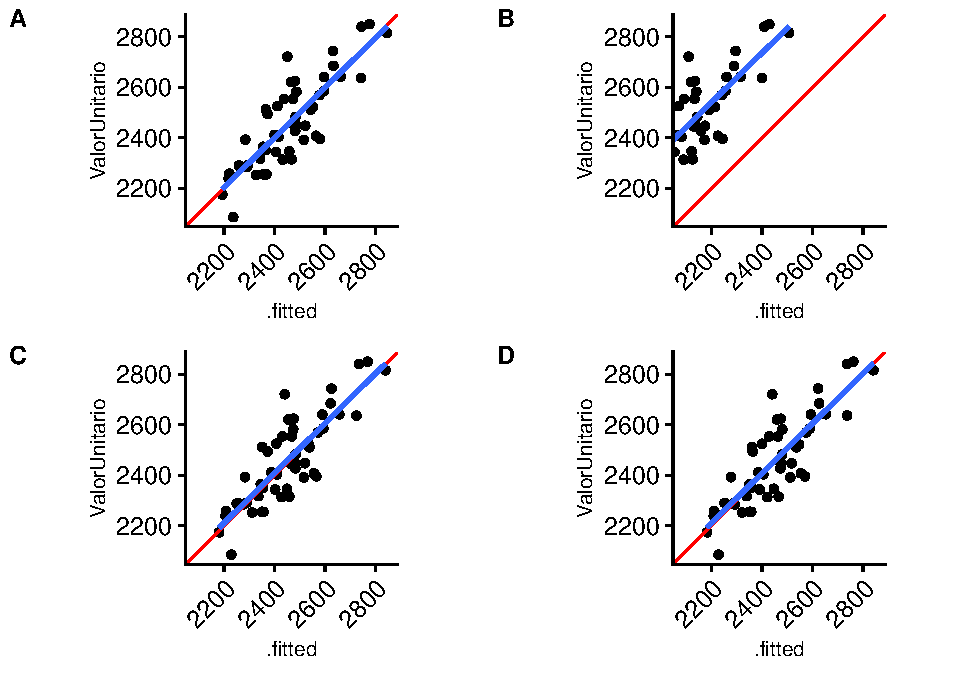
\includegraphics[width=1\linewidth]{EstudoCaso_files/figure-latex/powerPlots-1} 

}

\caption{Gráficos de poder de predição para cada modelo.}\label{fig:powerPlots}
\end{figure}

\end{document}
